\FloatBarrier

Um die Oberflächengüte des Rheniumkristalls zu analysieren, wurde die Oberfläche zunächst mit LEED
untersucht. Zuvor wurde die Probe geflasht bei einer Hochspannung von 700V und einem Strom
von 150mA zwischen Filament und Probe, was etwa einer Temperatur von \ldots entspricht.\\
Rhenium hat eine hcp-Kristallstrukur, daher erwartet man auch als Beugungsmuster an der Oberfläche
eine hexagonale Periodizität. Zwar ist das LEED-Beugungsbild eine direkte Abbildung des reziproken
Raums, nicht des Realraums, doch ist das reziproke Gitter einer hcp-Struktur wiederum eine
hcp-Struktur.\\
Bei einer Elektronenergie von 208eV ergaben sich Beugungsmuster wie in Abb. \ref{rekristall}. Es
zeigte sich, dass die Oberfläche keine homogene Güte besitzt. In den äußeren Bereichen des Kristalls
ist die Struktur gekennzeichnet durch scharfe Spots und ein gleichmäßiges, hexagonales Muster, was
auf eine periodische, planare Oberfläche hinweist. In der Mitte des Kristalls jedoch besitzt die
Oberfläche eine unregelmäßige Struktur; die Hauptspots heben sich kaum von den ungleich verteilen
Spots der Überstruktur ab. \\
Da zur Vermutung stand, diese Überstruktur könnte wie bei Wolfram von Kohlenstoffverunreinigungen
herrühren, wurde der Kristall unter einer Sauerstoffatmossphäre von etwa $10^{-8}$mbar bei einer
Temperatur von ungefähr \ldots K geglüht. Dabei sollte der Kohlenstoff mit dem Sauerstoff zu
Kohlenmonoxid reagieren, welches durch Flashen von der Oberfläche entfernt werden kann. Dies
resultierte hier jedoch in keiner wesentlichen Verbesserung, sodass bei den folgenden LEED- sowie STM-Messungen
nur die äußeren Bereiche des Kristalls berücksichtigt wurden.\\


\begin{figure}[htbp]
	\begin{minipage}[b]{0.5\textwidth} 
		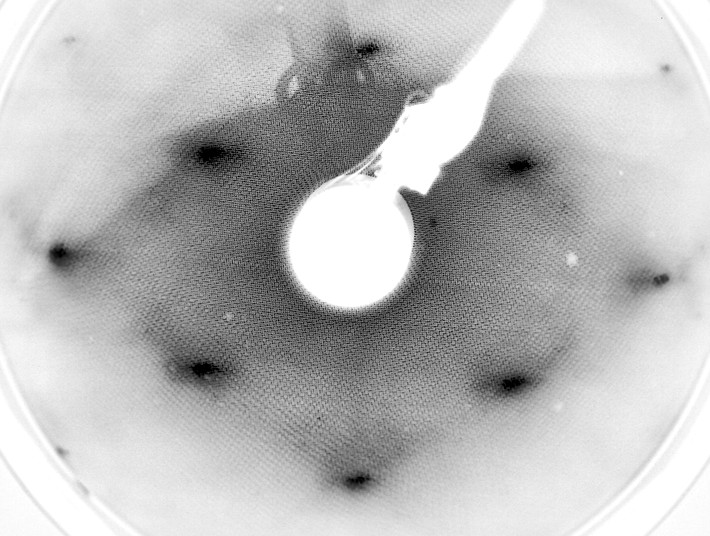
\includegraphics[width=\textwidth]{LEED-Bilder/bearbeitet/unbedampft_E207}
	\end{minipage}
	\hfill
	\begin{minipage}[b]{0.5\textwidth}
		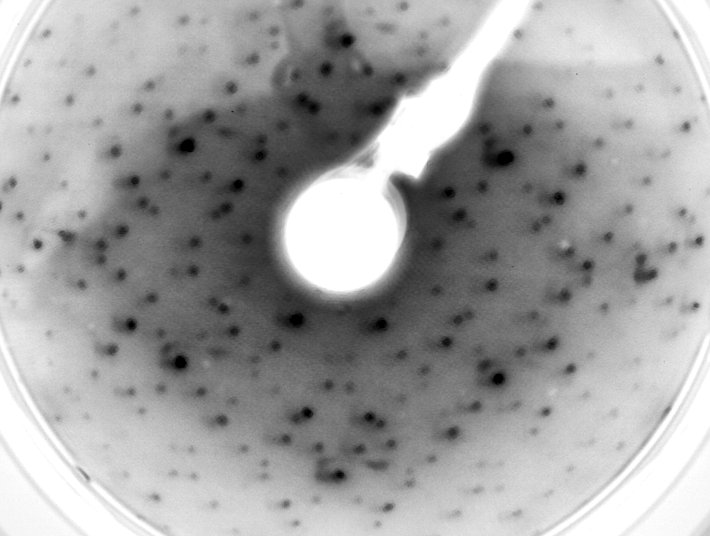
\includegraphics[width=\textwidth]{LEED-Bilder/bearbeitet/unbedampft_E207_MitteKristall.jpg}
	\end{minipage}
	\caption{\textit{Links der Re-Kristall mit scharfen Spots und eindeutiger Struktur. Rechts die
	Re-Oberfläche mit Verschmutzung, zu erkennen an der Überstruktur und den schwächeren Hauptspots.}}
	\label{rekristall} 
\end{figure}

Das Wachstum von Gold auf der Rheniumoberfläche wurde nun zuerst durch LEED für
verschiedene Bedeckungsgrade des Kristalls untersucht. Dazu wurden eine halbe, eine, sechs, zehn und
30 Monolagen auf den Kristall aufgedampft und die Beugungsmuster miteinander verglichen. Die
entstandenen Aufnahmen sind in den Abbildungen \ref{1/2ML} bis \ref{30ML} zu sehen; zum Vergleich
ist auch noch eine Abbildung der unbedampften Probenoberfläche zu sehen. Alle Bilder entstanden
bei einer Elektronenenergie von 208eV.\\
Zu erkennen ist eine deutliche Abschwächung der Intensität und der Schärfe (?) beim Aufbringen einer
halben Monolage Gold im Vergleich zum unbedampften Kristall. Auch bei anderen Energien des
Elektronenstrahls war kein deutlicheres Beugungsmuster zu erhalten. Daraus lässt sich schließen,
dass die aufgebrachten Goldatome kein pseudomorphes Wachstum betreiben, d.h. sich nicht periodisch
auf das Oberflächengitter des Substrats absetzen und dieses damit fortführen. Die vorhandenden Spots
stammen von der Substratoberfläche, an der tiefer eindringende Elektronen gestreut werden. Bei einer
aufgedampften Monolage verringert sich die Intensität der Spots noch weiter; die Goldatome bilden
offensichtlich bei dieser Schichtdicke noch keine erkennbare Periodizität aus. Der Anteil der am
Substrat gestreuten Elektronen wird allerdings geringer, da nun die doppelte Anzahl von Goldatomen
die Elektronen am tieferen Eindringen und Rückstreuen hindern.\\
Ab sechs Monolagen Gold ist bis 30 Monolagen eine Steigerung der Intensität und der Schärfe zu
erkennen. Das Gold bildet nun eine eigene periodische Struktur aus, die Substratoberfläche trägt
bei diesen Schichtdicken nur noch unwesentlich bzw. gar nicht mehr zum Beugungsbild bei. Das
Oberflächengitter der Adatome besitzt wiederum eine hexagonales Periodizität. Obwohl Gold
prinzipiell eine kubisch-flächenzentrierte Struktur besitzt, rekonstruiert die 

\begin{figure}[htbp]
		\captionsetup{name=Abb.}
	\begin{minipage}[b]{0.5\textwidth} 
		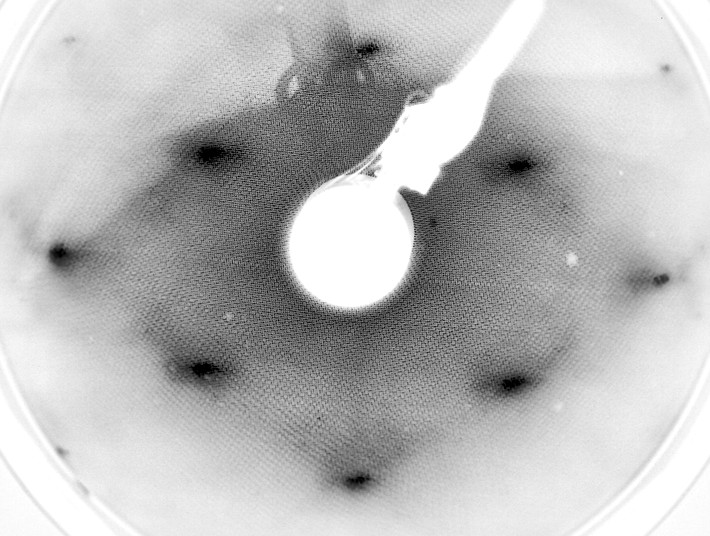
\includegraphics[width=\textwidth]{LEED-Bilder/bearbeitet/unbedampft_E207}
		\caption{\textit{Re-Oberfläche}}
		\label{0ML} 
	\end{minipage}
	\hfill
	\begin{minipage}[b]{0.5\textwidth}
		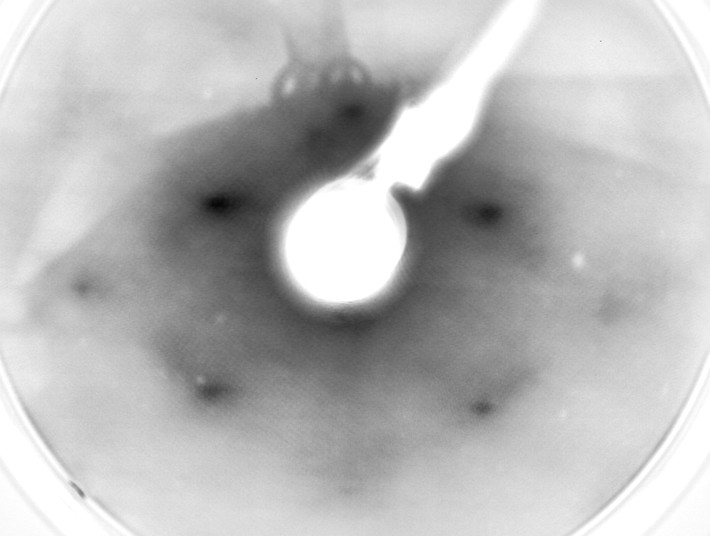
\includegraphics[width=\textwidth]{LEED-Bilder/bearbeitet/0_5ML_E208}
		\caption{\textit{1/2 Monolage Au}}
		\label{1/2ML} 
	\end{minipage}
	
	\begin{minipage}[b]{0.5\textwidth} 
		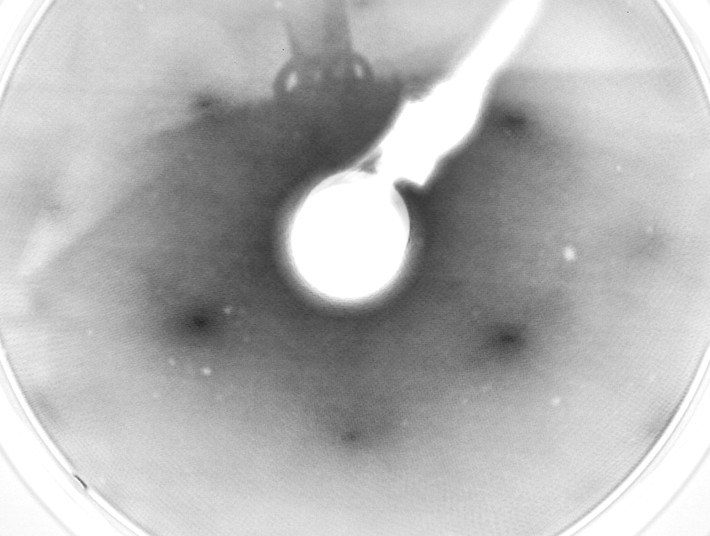
\includegraphics[width=\textwidth]{LEED-Bilder/bearbeitet/1ML_E207}
		\caption{\textit{1 Monolage Au}}
		\label{1ML} 
	\end{minipage}
	\hfill
	\begin{minipage}[b]{0.5\textwidth}
		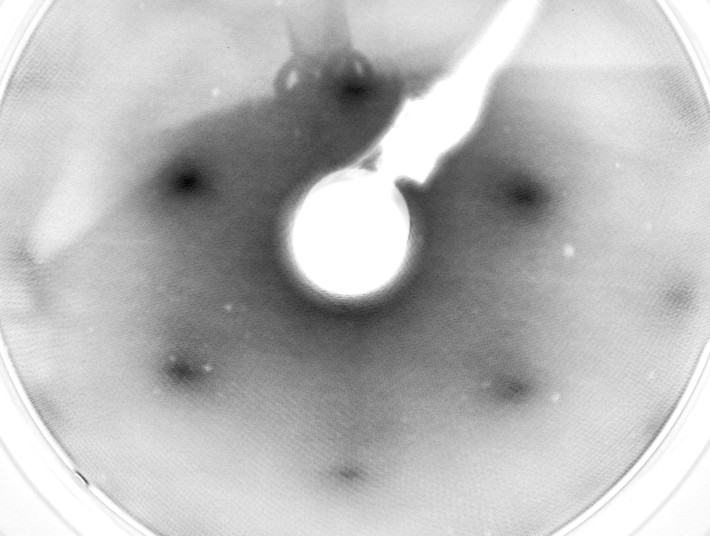
\includegraphics[width=\textwidth]{LEED-Bilder/bearbeitet/6ML_E207}
		\caption{\textit{6 Monolagen Au}}
		\label{6ML} 
	\end{minipage}
	
	\begin{minipage}[b]{0.5\textwidth} 
		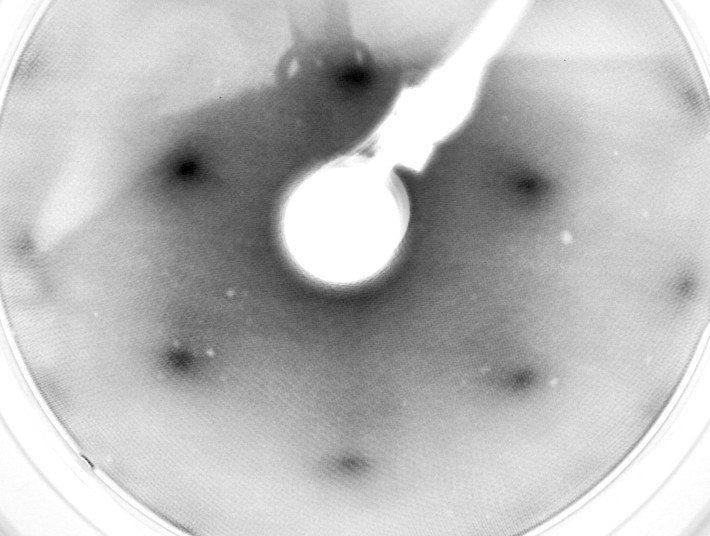
\includegraphics[width=\textwidth]{LEED-Bilder/bearbeitet/10ML_E207}
		\caption{\textit{10 Monolagen Au}}
		\label{10ML} 
	\end{minipage}
	\hfill
	\begin{minipage}[b]{0.5\textwidth}
		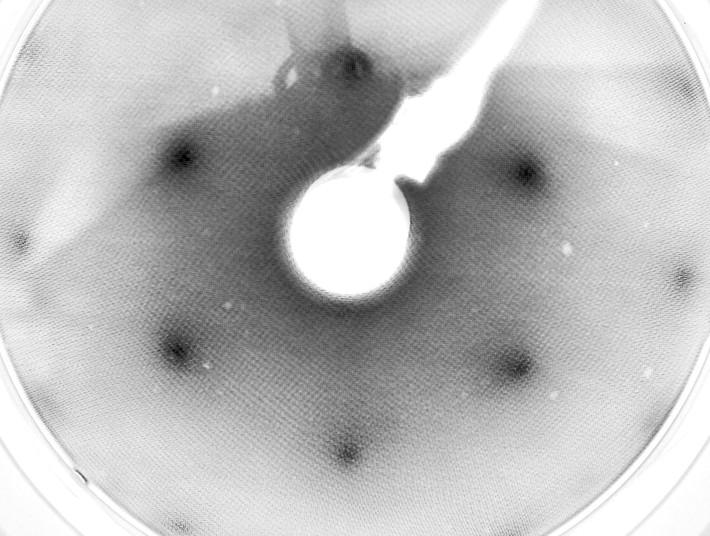
\includegraphics[width=\textwidth]{LEED-Bilder/bearbeitet/30ML_E208}
		\caption{\textit{30 Monolagen Au}}
		\label{30ML} 
	\end{minipage}
	\caption*{\textbf{Abb. 1.5-1.10:} \textit{LEED-Aufnahmen vom Re-Kristall ohne und mit
	verschiedenen Bedeckungsgraden von Gold.}}
\end{figure}


\FloatBarrier